\clearpage
\appendix
\section*{Appendix}
% \setcounter{page}{1}

This supplementary material provides additional details on the proposed method and experimental results that could not be included in the main manuscript due to page limitations.
Specifically, this appendix is organized as follows.

\begin{itemize}[left=1em]
\item Sec.~\ref{sec1} presents additional details of the models and training strategies. 
\item Sec.~\ref{sec2} presents details of training datasets and evaluation benchmarks.
\item Sec.~\ref{sec3} presents comprehensive experimental results on the performance of FlagScale~\cite{FlagScale2024}.
\end{itemize}


\section{Details of Models and Training}
\label{sec1}

RoboBrain-1.5-OS represents a significant advancement in robotic vision-language models, building upon the robust foundation of Qwen2.5-VL-7B~\cite{Qwen2.5-VL} through an elaborate three-stage training paradigm designed to progressively enhance both general and domain-specific capabilities.
(1) In Stage 1, the model undergoes full-parameter supervised fine-tuning (SFT) using 3M high-quality general VLM datasets with a learning rate of 1e-4, trained across 20 servers each equipped with 8$\times$A800 GPUs, aiming to establish robust foundational visual understanding and reasoning capabilities. (2) Stage 2 focuses on the robotics domain, utilizing 2.3M carefully curated robotic-related training data while retaining 10\% of Stage 1 data to prevent catastrophic forgetting. The learning rate is reduced to 1e-5 to ensure stable convergence. (3) The final Stage 3 specializes in optimization for RoboOS, first performing SFT with 245K OS-SFT samples (containing 2\% Stage 1 and 3\% Stage 2 data), followed by Group Relative Preference Optimization (GRPO)~\cite{shao2024grpo} using 4K OS-RL samples (only tool-calling samples), leveraging reinforcement learning (RL) for its efficiency and scalability. The GRPO phase in Stage 3 further reduces the learning rate to 1e-6, and completes training in 3 epochs on a single 8$\times$A800 server. The entire training process employs the DeepSpeed Zero3~\cite{zero} optimization strategy, with carefully configured key parameters including batch size (2 for SFT, 1 for GRPO), maximum sequence length (32768 for SFT, 8192 for GRPO), and weight decay (0.1). The number of completion (4) and maximum completion length (512) are specific for GRPO. Detailed hyperparameters are provided in Tab.~\ref{tab:training_setting}. This training scheme significantly enhances the model's performance in robotics applications and system compatibility while preserving the original capabilities of Qwen2.5-VL-7B~\cite{Qwen2.5-VL}.

\begin{table*}[!ht]
    \centering
    \caption{Detailed configuration for each training stage of the RoboBrain-1.5-OS.}
    \vspace{0.2cm}
    \label{tab:training_setting}
    \setlength{\tabcolsep}{12pt}
    \renewcommand{\arraystretch}{1.2}
    \resizebox{0.93\textwidth}{!}{%
    \begin{tabular}{@{}ll|c|c|c|c@{}}
        \toprule
        & & \textbf{Stage-1} & \textbf{Stage-2} & \multicolumn{2}{c}{\textbf{Stage-3}} \\ \cmidrule(l){3-3} \cmidrule(l){4-4} \cmidrule(l){5-6}
        & & \textbf{SFT} & \textbf{SFT} & \textbf{SFT} & \textbf{GRPO} \\
        \midrule 
        \multirow{2}{*}{\rotatebox[origin=c]{90}{\small \textit{Data}}}
        & \textbf{Dataset}  & General VLM & Robotic & OS-SFT (Part 1) & OS-RL (Part 2) \\
        & \#Samples & 3M & 2.3M & 245K & 4K \\
        \midrule 
        \multirow{2}{*}{\rotatebox[origin=c]{90}{\small \textit{Model}}}
        & \textbf{Trainable Part} & Full Model & Full Model & Full Model & Full Model \\
        & \#Tunable Parameters & 8.29B & 8.29B & 8.29B & 8.29B \\
        \midrule 
        \multirow{14}{*}{\rotatebox[origin=c]{90}{\small \textit{Training}}}
        & \textbf{Per-device Batch Size} & 2 & 2 & 4 & 1 \\
        & \textbf{Gradient Accumulation} & 2 & 2 & 2 & 2 \\   
        & \textbf{LR: $\{\psi_v^{\text{ViT}}, \phi_v^{\text{LLM}}\}$} & 1$\times 10^{-4}$ & 1 $\times 10^{-6}$ & 1 $\times 10^{-5}$ & 1 $\times 10^{-6}$ \\
        & \textbf{Epoch} & 1 & 1 & 1 & 3 \\
        & \textbf{Optimizer} & AdamW & AdamW & AdamW & AdamW \\
        & \textbf{Deepspeed} & Zero3 & Zero3 & Zero3 & Zero3 \\
        & \textbf{Weight Decay} & 0.1 & 0.1 & 0.1 & 0.0 \\
        & \textbf{Warmup Ratio} & 0.03 & 0.03 & 0.03 & 0.00 \\
        & \textbf{LR Schedule} & Cosine & Cosine & Cosine & Cosine \\
        & \textbf{Max Seq. Length} & 32768 & 32768 & 32768 & 8192 \\
        & \textbf{Max Compl. Length} & -- & -- & -- & 512 \\
        & \textbf{Num. of Compl.} & -- & -- & -- & 4 \\
        & \textbf{GPU Nums} & 20 $\times$ 8 & 20 $\times$ 8 & 4 $\times$ 8 & 1 $\times$ 8 \\
        \bottomrule
    \end{tabular}
    }
    \vspace{1mm}
    \vspace{-0.5em}
\end{table*}

\section{Details of Datasets and Benchmarks}
\label{sec2}

\subsection{Training Datasets}
The training of RoboBrain-1.5-OS leverages three comprehensive dataset categories: general VLM datasets for foundational capabilities, Robotic datasets for embodied intelligence, and RoboOS-Enhanced datasets for system-specific optimization.
The specific composition of these three datasets are listed as follows:

\begin{itemize}[left=1em]
    \item \textbf{General VLM Datasets} (Total: 3M samples) – We systematically organized five specialized subsets to establish fundamental capabilities:  
    (1) \textit{General-873k}, curated from LRV-400K~\cite{,liu2023mitigating} and LLaVA-665K~\cite{li2024llavaov} through rigorous filtering and restructuring, enhances broad question-answering with diverse QA pairs spanning descriptive, analytical, and inferential tasks.  
    (2) \textit{ScanView-318k} integrates multimodal 3D scene understanding data from MMScan-224K~\cite{mmscan} (annotated object segmentation and textual descriptions), 3RScan-43K~\cite{3rscan} (3D reconstructions with semantic labels), ScanQA-25K~\cite{scanqa} (QA pairs grounded in 3D environments), and SQA3D-26K~\cite{sqa3d} (spatial QA), enabling fine-grained environmental perception.  
    (3) \textit{VG-326k} combines Ref-L4~\cite{chen2024revisiting} (45K expressions spanning 365 object categories), OV-VG~\cite{li2024llavaov} (visual grounding smaples in Llava-OneVision), RefCOCO/RefCOCO+~\cite{yu2016modeling,mao2016generation} (natural language descriptions with restrictive/non-restrictive spatial constraints), and Visual Genome~\cite{krishna2017visual} (rich region descriptions and relational annotations) for precise visual grounding and localization.  
    (4) \textit{Spatial-R-1005k} leverages Ref-Reasoning-791K~\cite{yang2020graph} (complex expressions with attribute/spatial reasoning and adversarial images), COPS-Ref-148K~\cite{chen2020cops}, and Spatial-Trans-66K~\cite{tan2025reason} to model compositional relationships.  
    (5) \textit{Temporal-R-525k} synthesizes Embodied-Reasoner-9K~\cite{zhang2025embodied}, HandMeThat-300K~\cite{wan2022handmethat} (abstract command-based planning), and 200K+ simulated reasoning samples for sequential event comprehension. All datasets underwent deduplication and quality filtering to balance capability coverage while eliminating noise.

    \item \textbf{Robotic Datasets} (Total: 2.3M samples) – Designed to develop four core embodied intelligence competencies:  
    (1) \textit{Planning-700k} aggregates RoboVQA-Clean-200K (reconstructed from original RoboVQA-800K~\cite{sermanet2024robovqa}), ShareRobot-Plan-400K (a planning subset of ShareRobot~\cite{ji2025robobrain}), RoboBench-50K (constructed based on real-world embodied tasks by ourselves), and AgiBotWorld-Alpha-50K~\cite{bu2025agibot} to train hierarchical task decomposition and long-horizon planning.  
    (2) \textit{Pointing-537k} unifies Object-Ref-347K~\cite{yuan2024robopoint} (287K images with coordinate-based QA) and Pixmo-Point-190K~\cite{deitke2024molmo} (indoor scene point annotations) to refine spatial awareness via coordinate regression.  
    (3) \textit{Affordance-373k} merges Region-Ref-320K~\cite{yuan2024robopoint} (270K images with interactive region QA), PACO-LVIS-45K~\cite{ramanathan2023paco} (object functionality labels), and ShareRobot-Affordance-8K~\cite{ji2025robobrain} to predict actionable object properties.  
    (4) \textit{Trajectory-428k} combines LLaRVA-420K~\cite{niu2024llarva} and ShareRobot-Trajectory-8K~\cite{yuan2024robopoint} to learn manipulation sequences for successful execution. Each subset was iteratively optimized for robotic applicability, emphasizing precision in action-object mapping. To mitigate catastrophic forgetting while maintaining model performance, we implement a knowledge retention strategy where 10\% of Stage 1 training samples (Stage1-300K) are preserved during Stage 2.

    \item \textbf{RoboOS-Enhanced Datasets} (Total: 249k samples) – Tailored for RoboOS integration:  
    (1) \textit{Multi-Robot-45k} features 68 collaboration task types (supermarket/household/restaurant scenarios) generated via DeepSeek-V3-0324~\cite{liu2024deepseek}, with scene graphs, robot specs, and workflow visualizations for subtask reasoning.  
    (2) \textit{Robotic-Agent-144k} augments Multi-Robot-45k generated via DeepSeek-V3-0324~\cite{liu2024deepseek} with probabilistically sampled Observation-Action pairs (144K correct/error-injected variants) to improve operational robustness through SFT and RL training (140K for SFT and the rest for GRPO). This architecture ensures seamless adaptation to the RoboOS ecosystem implementation while preserving task-specific performance in multi-agent coordination and tool invocation.
\end{itemize}

\subsection{Evaluation Settings}
\textbf{Evaluation Baselines}
The reference baselines for comparison include: (1) Vision-Language Models (VLMs) of comparable parameter scales (e.g., LLaVA-OneVision-7B~\cite{li2024llavaov}, Qwen2.5-VL-7B~\cite{Qwen2.5-VL}, RoboBrain-7B-1.0~\cite{ji2025robobrain}, RoboPoint-14B~\cite{yuan2024robopoint}), and (2) larger general-purpose LLMs (e.g., Qwen3-14B~\cite{qwen3_2025}, DeepSeek-V3-685B~\cite{liu2024deepseek}). We evaluate vision-based and text-based benchmarks for VLMs, while only text-based benchmarks for LLMs. 

\textbf{Evaluation Benchmarks}
We conducted comprehensive evaluations on the model's four core robotic operation capabilities (Multi-Robot Planning, Pointing Prediction, Affordance Prediction, and Trajectory Prediction), with the benchmark configurations specified as follows:

\begin{itemize}[left=1em]
\item \textbf{Multi-Robot Planning} 
Our evaluation framework assesses multi-robot planning capabilities across three task scenarios: restaurant environments, commercial supermarkets, and household settings. Using RoboOS as the testbed system, we employ the Tool-Calling Accuracy Rate (AR) metric~\cite{zhang2024lmms} for quantitative assessment. For the three task scenarios of restaurant, supermarket, and household settings, we randomly sampled and generated 200 task samples for each scenario as a benchmark for testing. The task specifications for each scenario are shown in Fig.~\ref{fig:household}-\ref{fig:supermarket}. These samples are used to evaluate global task decomposition and agent-based tool-calling in RoboOS, with corresponding prompts illustrated in Fig.~\ref{fig:prompt1} and Fig.~\ref{fig:prompt2}.

\item \textbf{Pointing Prediction} 
We evaluate pointing prediction performance using the Where2Place dataset~\cite{yuan2024robopoint}, which contains 100 real-world images depicting cluttered environments with annotated spatial relations. Each image includes: (i) a textual description specifying desired free space, (ii) a ground-truth mask of the target region, and (iii) corresponding query points that probe the model's ability to localize referenced spaces. Performance is quantified through Hit Accuracy measured against target masks using the AR metric, assessing the precision of robotic systems in interpreting spatial references and predicting intended pointing locations.

\item \textbf{Affordance Prediction}
We utilize the AGD20K benchmark~\cite{luo2024grounded} - a comprehensive dataset comprising over 20,000 annotated images spanning diverse affordance categories - to evaluate the performance of affordance prediction. The evaluation protocol measures mean Average Precision (mAP) across multiple Intersection-over-Union (IoU) thresholds (0.25, 0.50, 0.75, 0.90), providing rigorous assessment of model robustness.

\item \textbf{Trajectory Prediction}
Our trajectory analysis employs the ShareRobot-Trajectory benchmark~\cite{ji2025robobrain} with three complementary metrics: 
(1) Discrete Fréchet Distance (DFD)~\cite{gu2023rt}: Computes the minimum leash length required for coupled traversal of predicted and ground-truth trajectories, capturing both geometric similarity and temporal alignment.
(2) Hausdorff Distance (HD): Measures worst-case positional deviation between trajectories.
(3) Root Mean Square Error (RMSE): Quantifies average pointwise Euclidean distance errors.
This multi-metric approach enables hierarchical analysis of trajectory quality, from global shape preservation (DFD) to local precision (RMSE), with HD identifying critical failure cases.

\end{itemize}

\section{Efficiency Performance on FlagScale}
\label{sec3}
This study conducts a comprehensive evaluation of the impact of FlagScale~\cite{FlagScale2024} on inference efficiency within the RoboOS framework through controlled comparative testing between two system configurations: RoboOS without FlagScale \textcolor{orange}{(Baseline)} and RoboOS with FlagScale  \textcolor{blue}{(+ FlagScale)}.

\subsection{Experimental Setup}
 All controlled comparative testing experiments were performed on an NVIDIA RTX 4090 GPU featuring 24GB of GDDR6X VRAM, noting that this hardware architecture lacks native support for FP8 tensor operations. The evaluation environment maintained strict parameter consistency, including fixed GPU memory utilization at 90\% through the gpu\_memory\_utilization=0.9 setting while deliberately disabling prefix caching to establish baseline performance measurements.
The experimental design incorporated several optimized computational parameters to ensure representative benchmarking conditions. These included a maximum sequence limit of 16 concurrent processes (max\_num\_seqs=16) and a progressive CUDA graph capture strategy configured for batch sizes [1, 2, 4, 8, 16], enabling efficient batch processing across varying workload demands. Primary performance metrics focused on End-to-Token Latency (E2TL) measurements for 85-token generation outputs, with particular attention to the characteristic disparity between initial batch latency and steady-state operational performance. The evaluation further examined scaling characteristics through Tensor Parallelism configurations at three distinct levels (TP1, TP2, and TP4) to assess both single-device and multi-device acceleration potential.



\subsection{FP16 Performance}
The FP16 latency comparisons demonstrate consistent acceleration benefits from FlagScale optimization across all tensor parallelism configurations. As shown in Tab.~\ref{tab:latency_comparison1}, the relative improvement decreases monotonically from 48.3\%–62.9\% at batch size of 1, to 16.4\%–20.8\% at batch size of 16 under TP1–TP4 configurations. This inverse correlation between batch size and optimization efficacy suggests diminishing returns for memory-bound operations at larger workloads. The non-linear latency growth pattern—where baseline latency increases 3.18× from batch 1 to 16 versus 5.14× for FlagScale—indicates superior batch processing scalability of the optimized implementation.

\begin{table}[h]
\centering
\caption{FP16 Latency Comparison (85-token generation, ms)}
\label{tab:latency_comparison1}
\resizebox{0.98\columnwidth}{!}{
\begin{tabular}{c|cc|cc|cc}
\toprule
\multirow{2}{*}{Batch Size} & \multicolumn{2}{c|}{E2TL-TP1} & \multicolumn{2}{c|}{TP2} & \multicolumn{2}{c}{TP4} \\
\cmidrule(lr){2-3} \cmidrule(lr){4-5} \cmidrule(lr){6-7}
 & \textcolor{orange}{Baseline} & \textcolor{blue}{+ FlagScale} & \textcolor{orange}{Baseline} & \textcolor{blue}{+ FlagScale} & \textcolor{orange}{Baseline} & \textcolor{blue}{+ FlagScale} \\
\midrule
1 & 4.06 & 2.10 (-48.3\%) & 3.85 & 1.52 (-60.5\%) & 3.29 & 1.22 (-62.9\%) \\
2 & 4.64 & 2.69 (-42.0\%) & 4.41 & 2.08 (-52.8\%) & 3.96 & 1.75 (-55.8\%) \\
4 & 5.79 & 3.83 (-33.9\%) & 5.24 & 3.16 (-39.7\%) & 4.95 & 2.78 (-43.8\%) \\
8 & 8.09 & 6.13 (-24.2\%) & 7.34 & 5.25 (-28.5\%) & 7.31 & 4.90 (-33.0\%) \\
16 & 12.92 & 10.80 (-16.4\%) & 12.16 & 9.63 (-20.8\%) & 11.21 & 9.11 (-18.7\%) \\
\bottomrule
\end{tabular}
}
\end{table}

\subsection{W8A16 Performance}
Quantization to W8A16 precision yields additional latency reductions beyond FP16 baselines, with FlagScale achieving 54.0\%–65.2\% improvement for single-query inference, as shown in Tab.~\ref{tab:latency_comparison2}. The TP4 configuration maintains the most significant gains across all batch sizes, demonstrating 23.4\%–65.2\% lower latency compared to baseline. Two key observations emerge: (1) The absolute latency values under W8A16 are consistently 12\%–17\% lower than corresponding FP16 results, confirming the expected quantization benefits; (2) The optimization maintains stable relative improvements across precision modes, with TP2 showing particularly consistent 20.0\%–60.5\% reductions. The convergence of latency values at batch size 16 (9.11–10.62ms across TP modes) suggests a hardware-bound limit for large-batch processing regardless of parallelism configuration.

\begin{table}[h]
\centering
\caption{W8A16 Latency Comparison (85-token generation, ms)}
\label{tab:latency_comparison2}
\resizebox{0.98\columnwidth}{!}{
\begin{tabular}{c|cc|cc|cc}
\toprule
\multirow{2}{*}{Batch Size} & \multicolumn{2}{c}{E2TL-TP1} & \multicolumn{2}{c}{TP2} & \multicolumn{2}{c}{TP4} \\
\cmidrule(lr){2-3} \cmidrule(lr){4-5} \cmidrule(lr){6-7}
& \textcolor{orange}{Baseline} & \textcolor{blue}{+ FlagScale} & \textcolor{orange}{Baseline} & \textcolor{blue}{+ FlagScale} & \textcolor{orange}{Baseline} & \textcolor{blue}{+ FlagScale} \\
\midrule
1  & 3.48 & 1.60 (-54.0\,\%) & 3.34 & 1.32 (-60.5\,\%) & 3.36 & 1.17 (-65.2\,\%) \\
2  & 4.17 & 2.22 (-46.8\,\%) & 4.21 & 1.91 (-54.6\,\%) & 3.92 & 1.69 (-56.9\,\%) \\
4  & 5.52 & 3.39 (-38.6\,\%) & 5.08 & 2.99 (-41.1\,\%) & 5.28 & 2.76 (-47.7\,\%) \\
8  & 7.78 & 5.78 (-25.7\,\%) & 7.46 & 5.25 (-29.6\,\%) & 6.96 & 4.84 (-30.5\,\%) \\
16 & 12.98 & 10.62 (-18.2\,\%) & 12.53 & 10.03 (-20.0\,\%) & 11.90 & 9.11 (-23.4\,\%) \\
\bottomrule
\end{tabular}
}
\end{table}


\begin{figure*}[!ht]
    \centering
   \vspace{-0.2cm}
    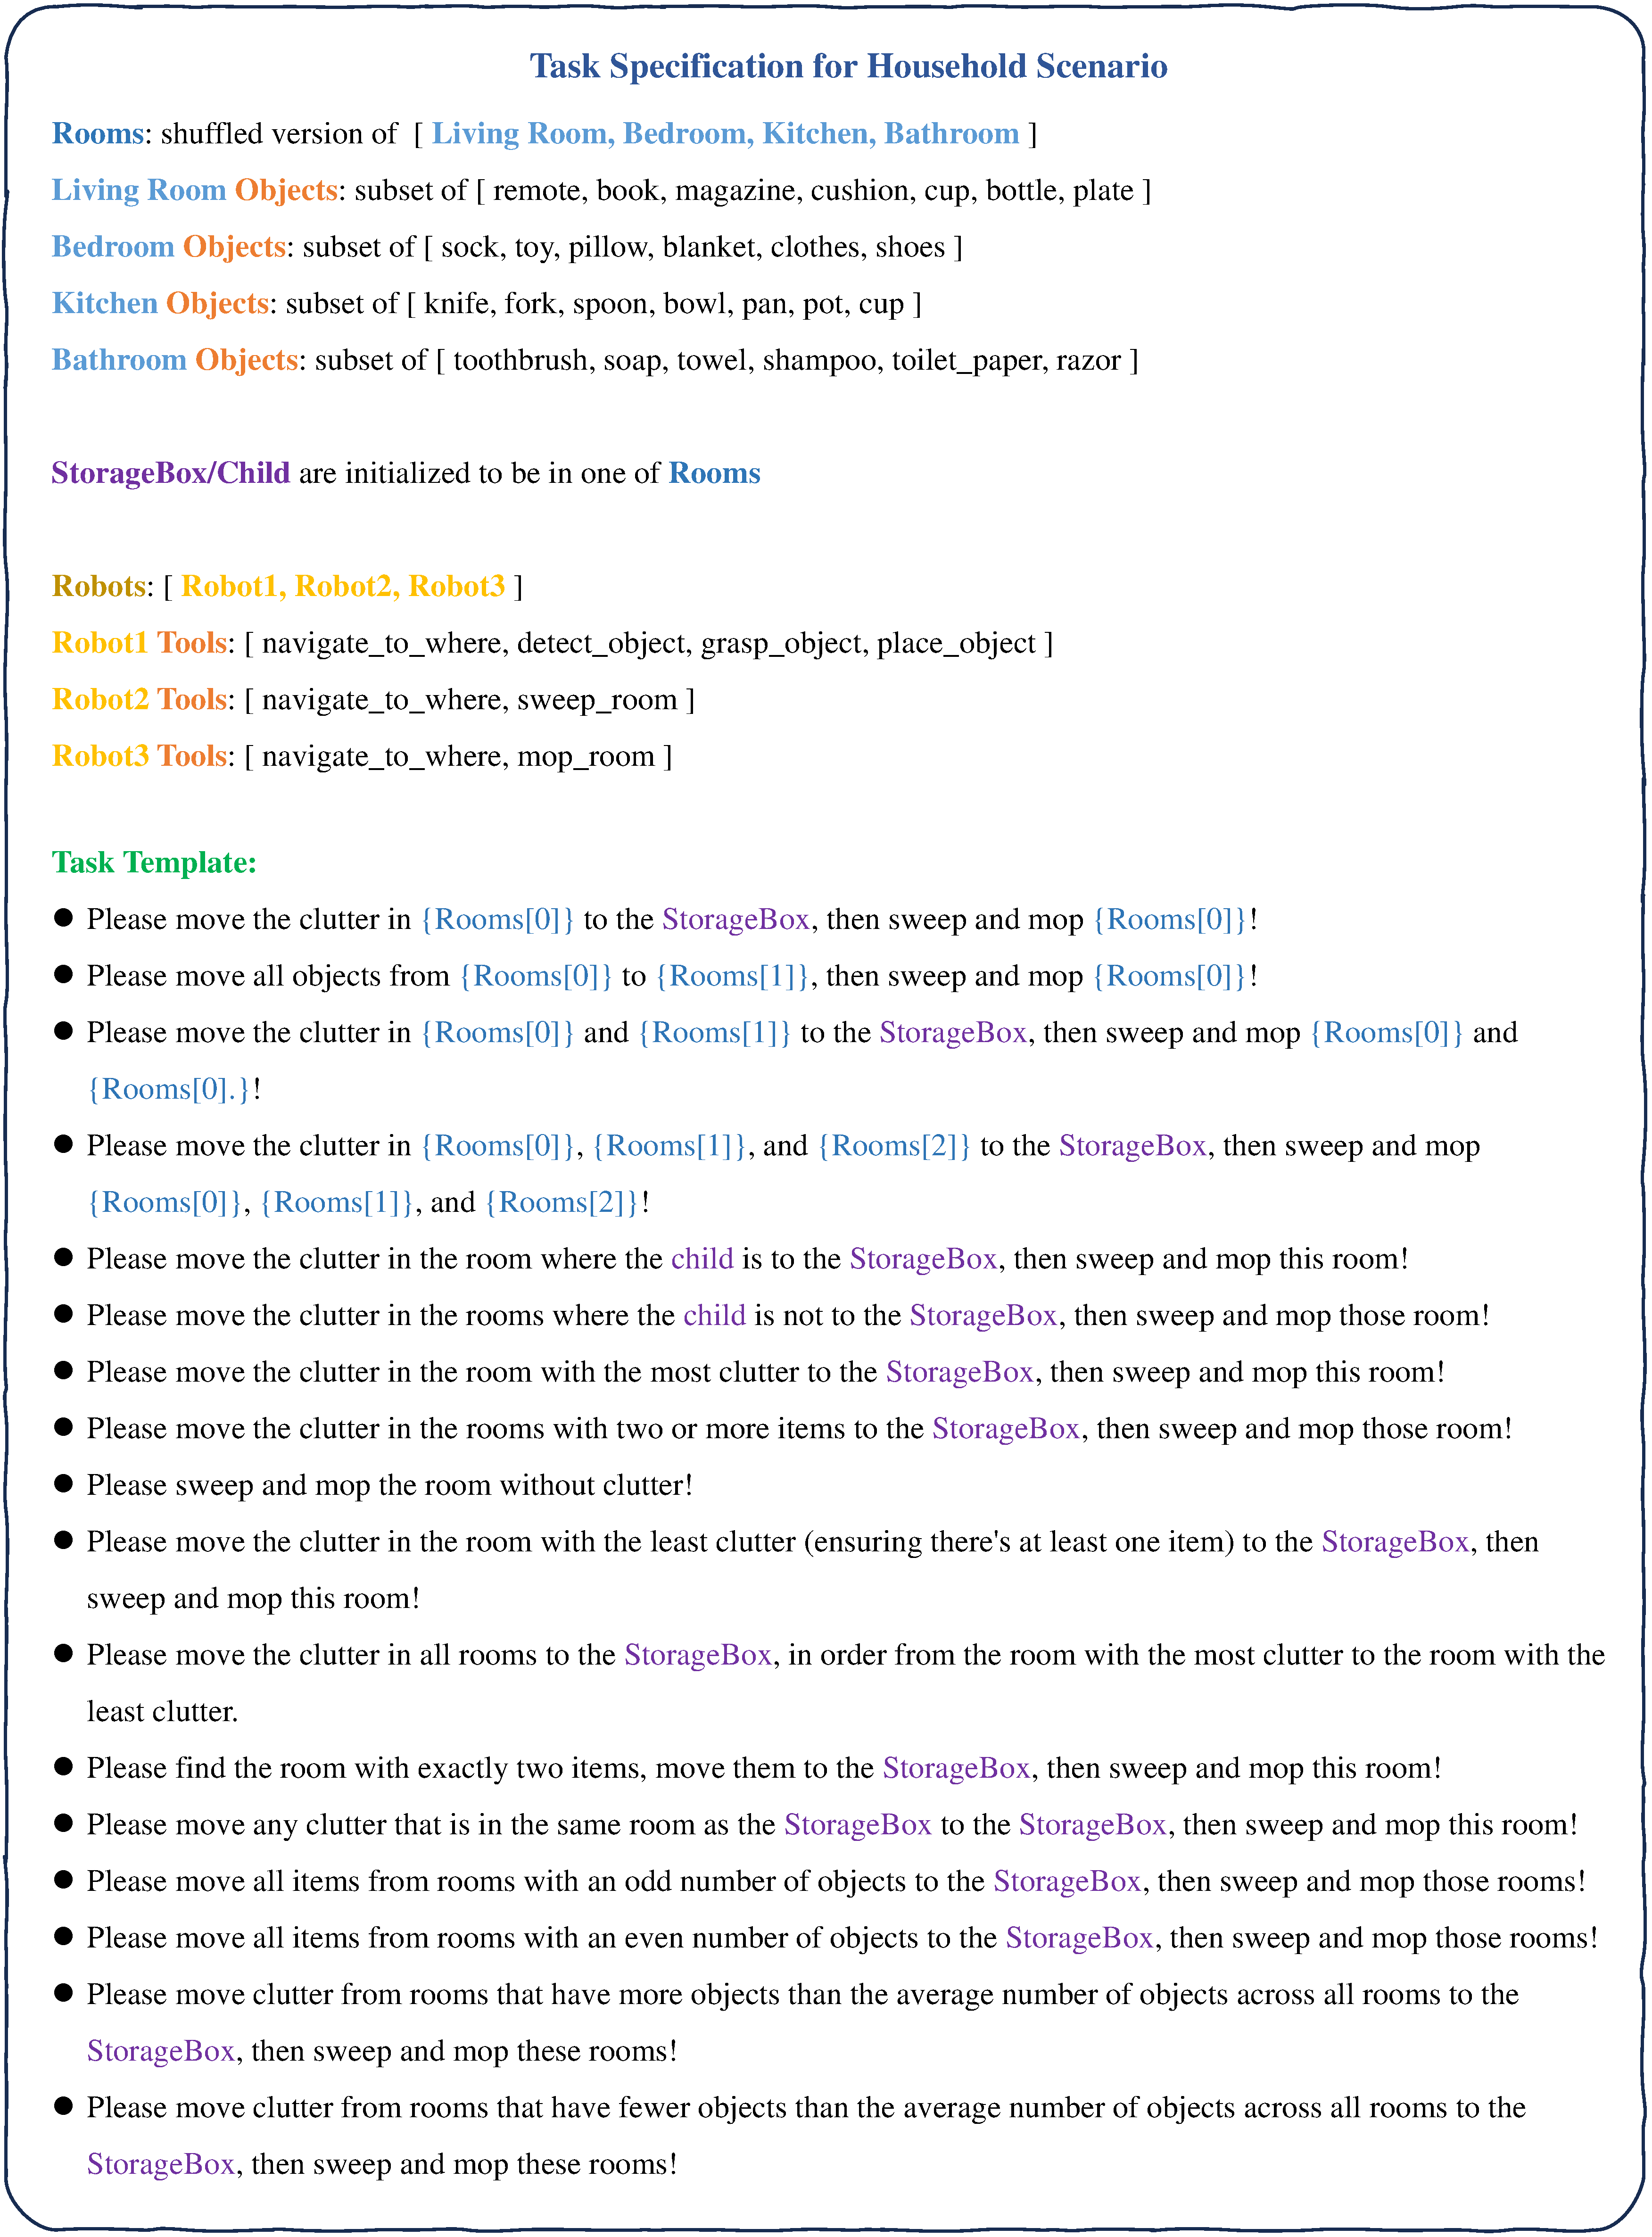
\includegraphics[width=0.93\linewidth]{images/household.pdf}
    \vspace{-0.25cm}
    \caption{
        Task specification for household scenario. 
        }
       \vspace{-0.5cm}
    \label{fig:household}
\end{figure*}

\begin{figure*}[!ht]
    \centering
   \vspace{-0.2cm}
    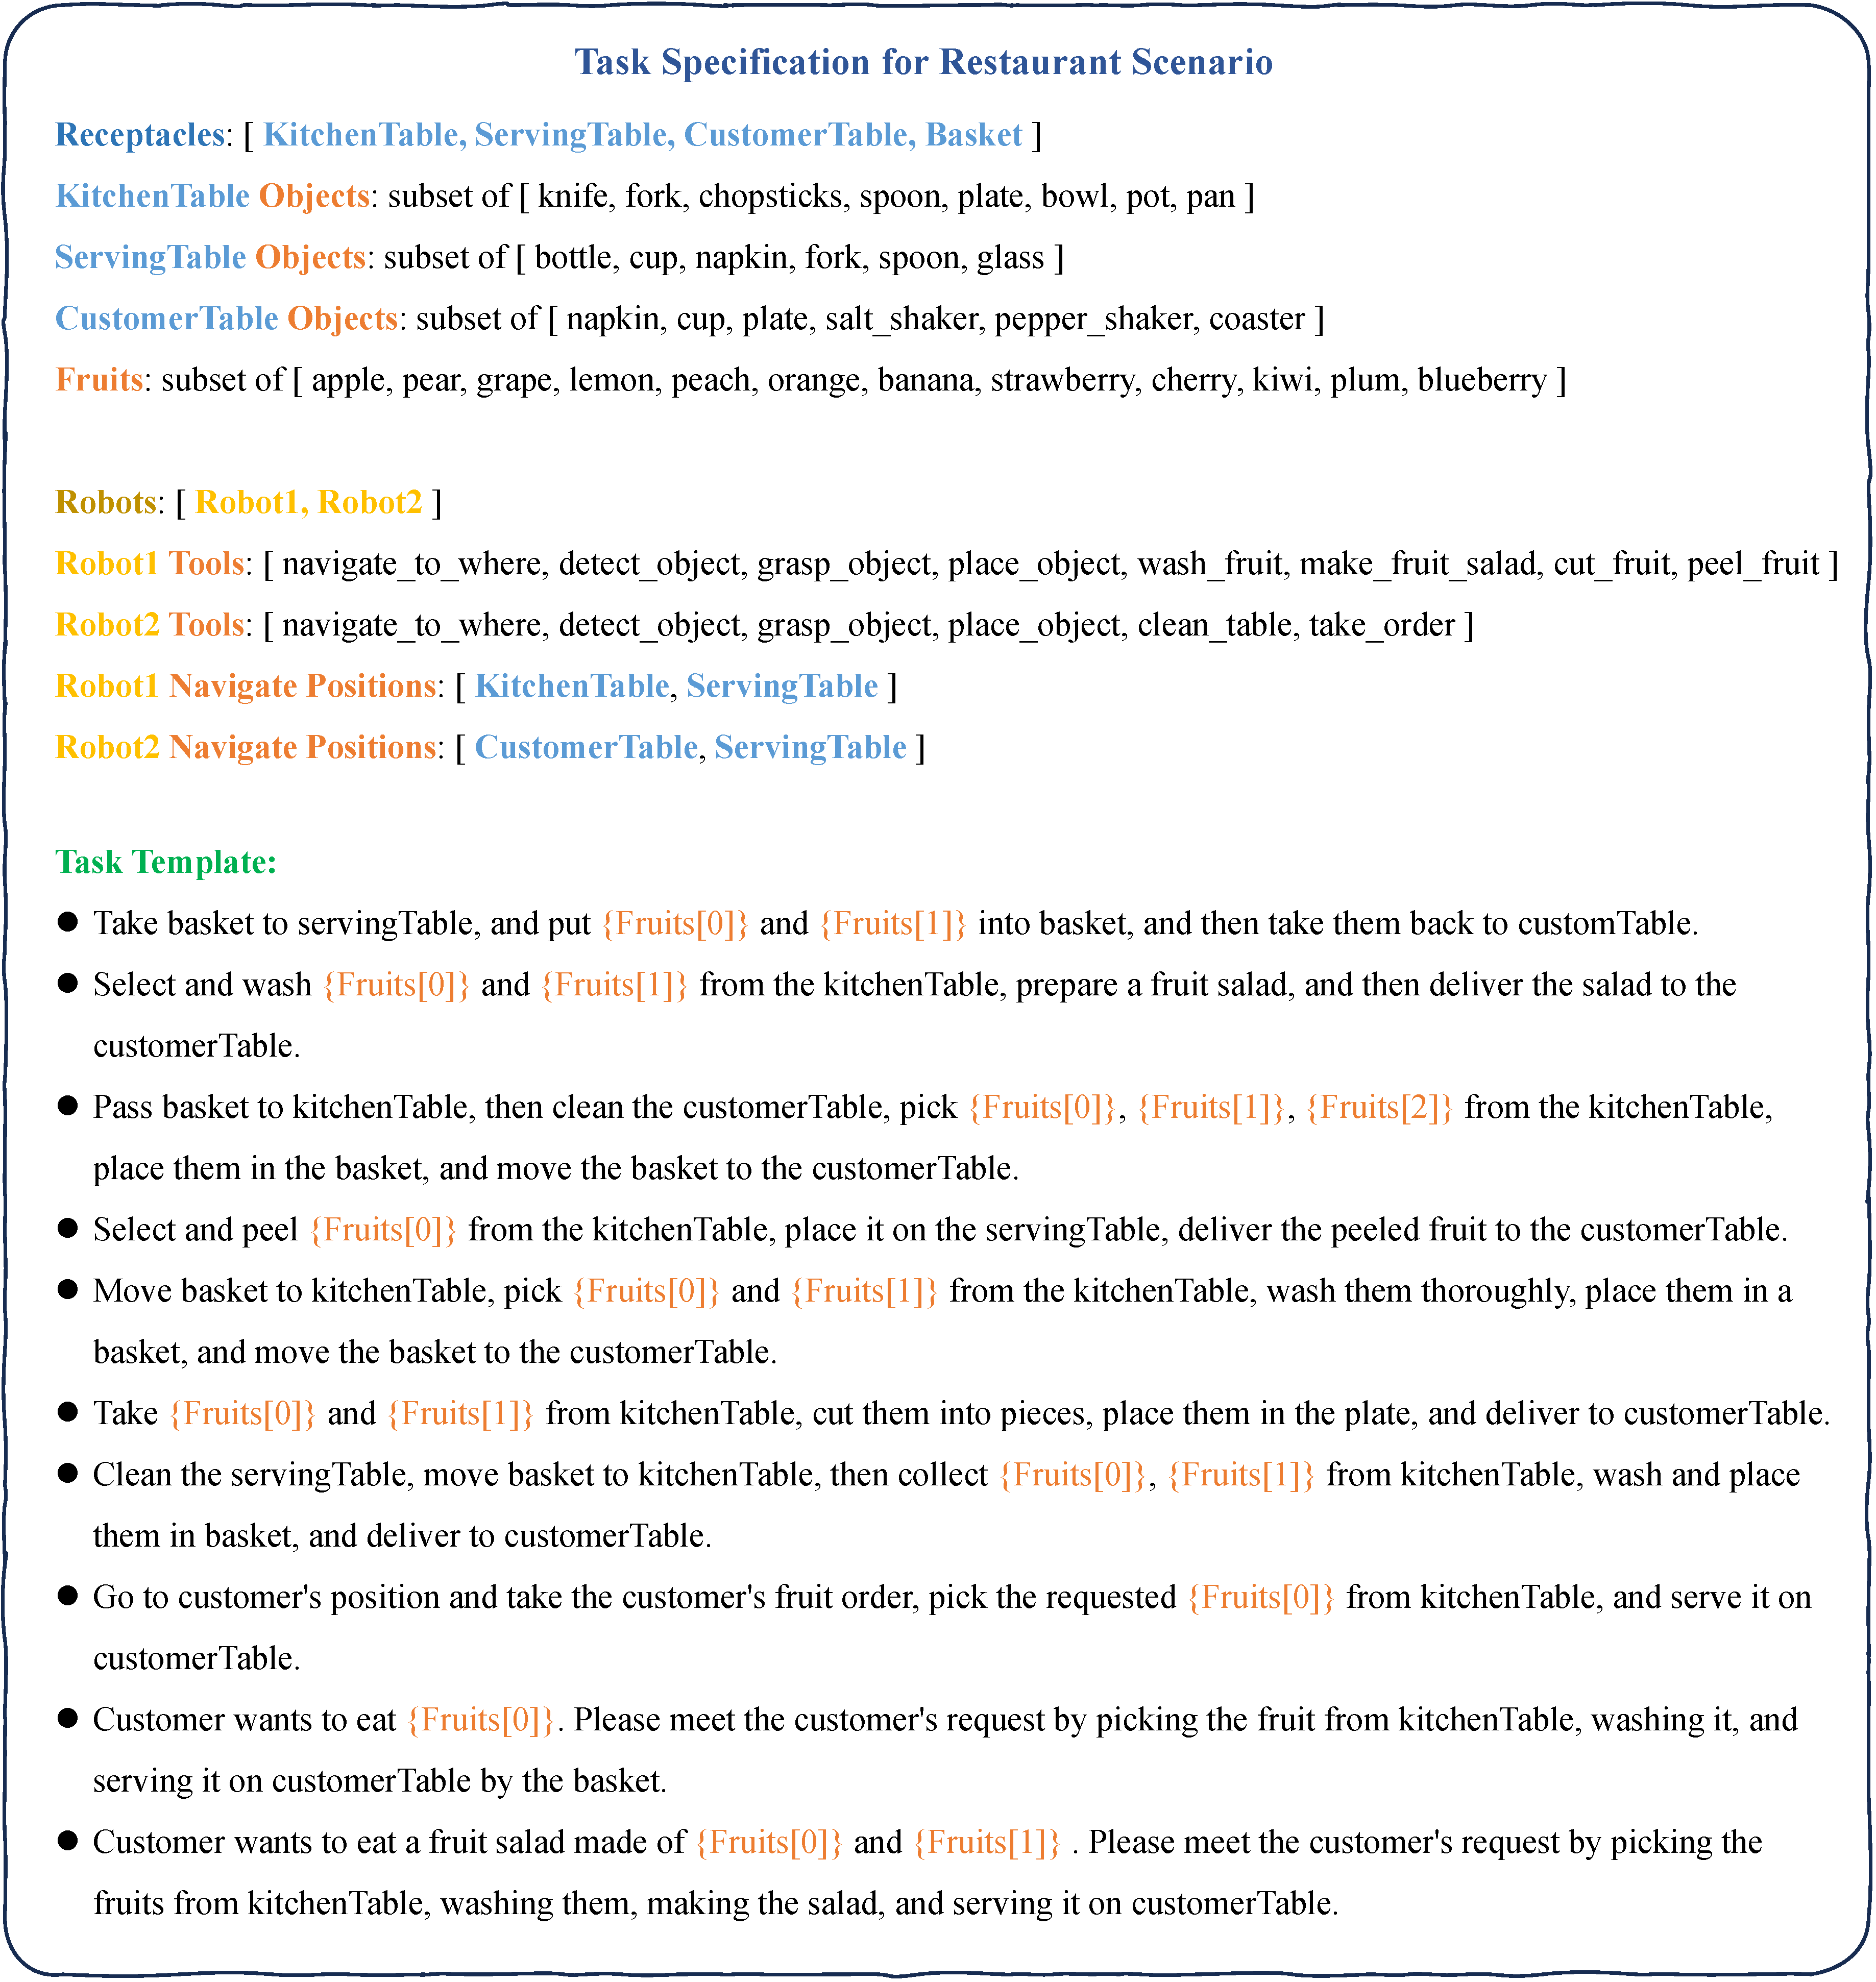
\includegraphics[width=0.94\linewidth]{images/restaurant.pdf}
    \vspace{-0.25cm}
    \caption{
        Task specification for restaurant scenario. 
        }
       \vspace{-0.5cm}
    \label{fig:restaurant}
\end{figure*}

\begin{figure*}[!ht]
    \centering
   \vspace{-0.2cm}
    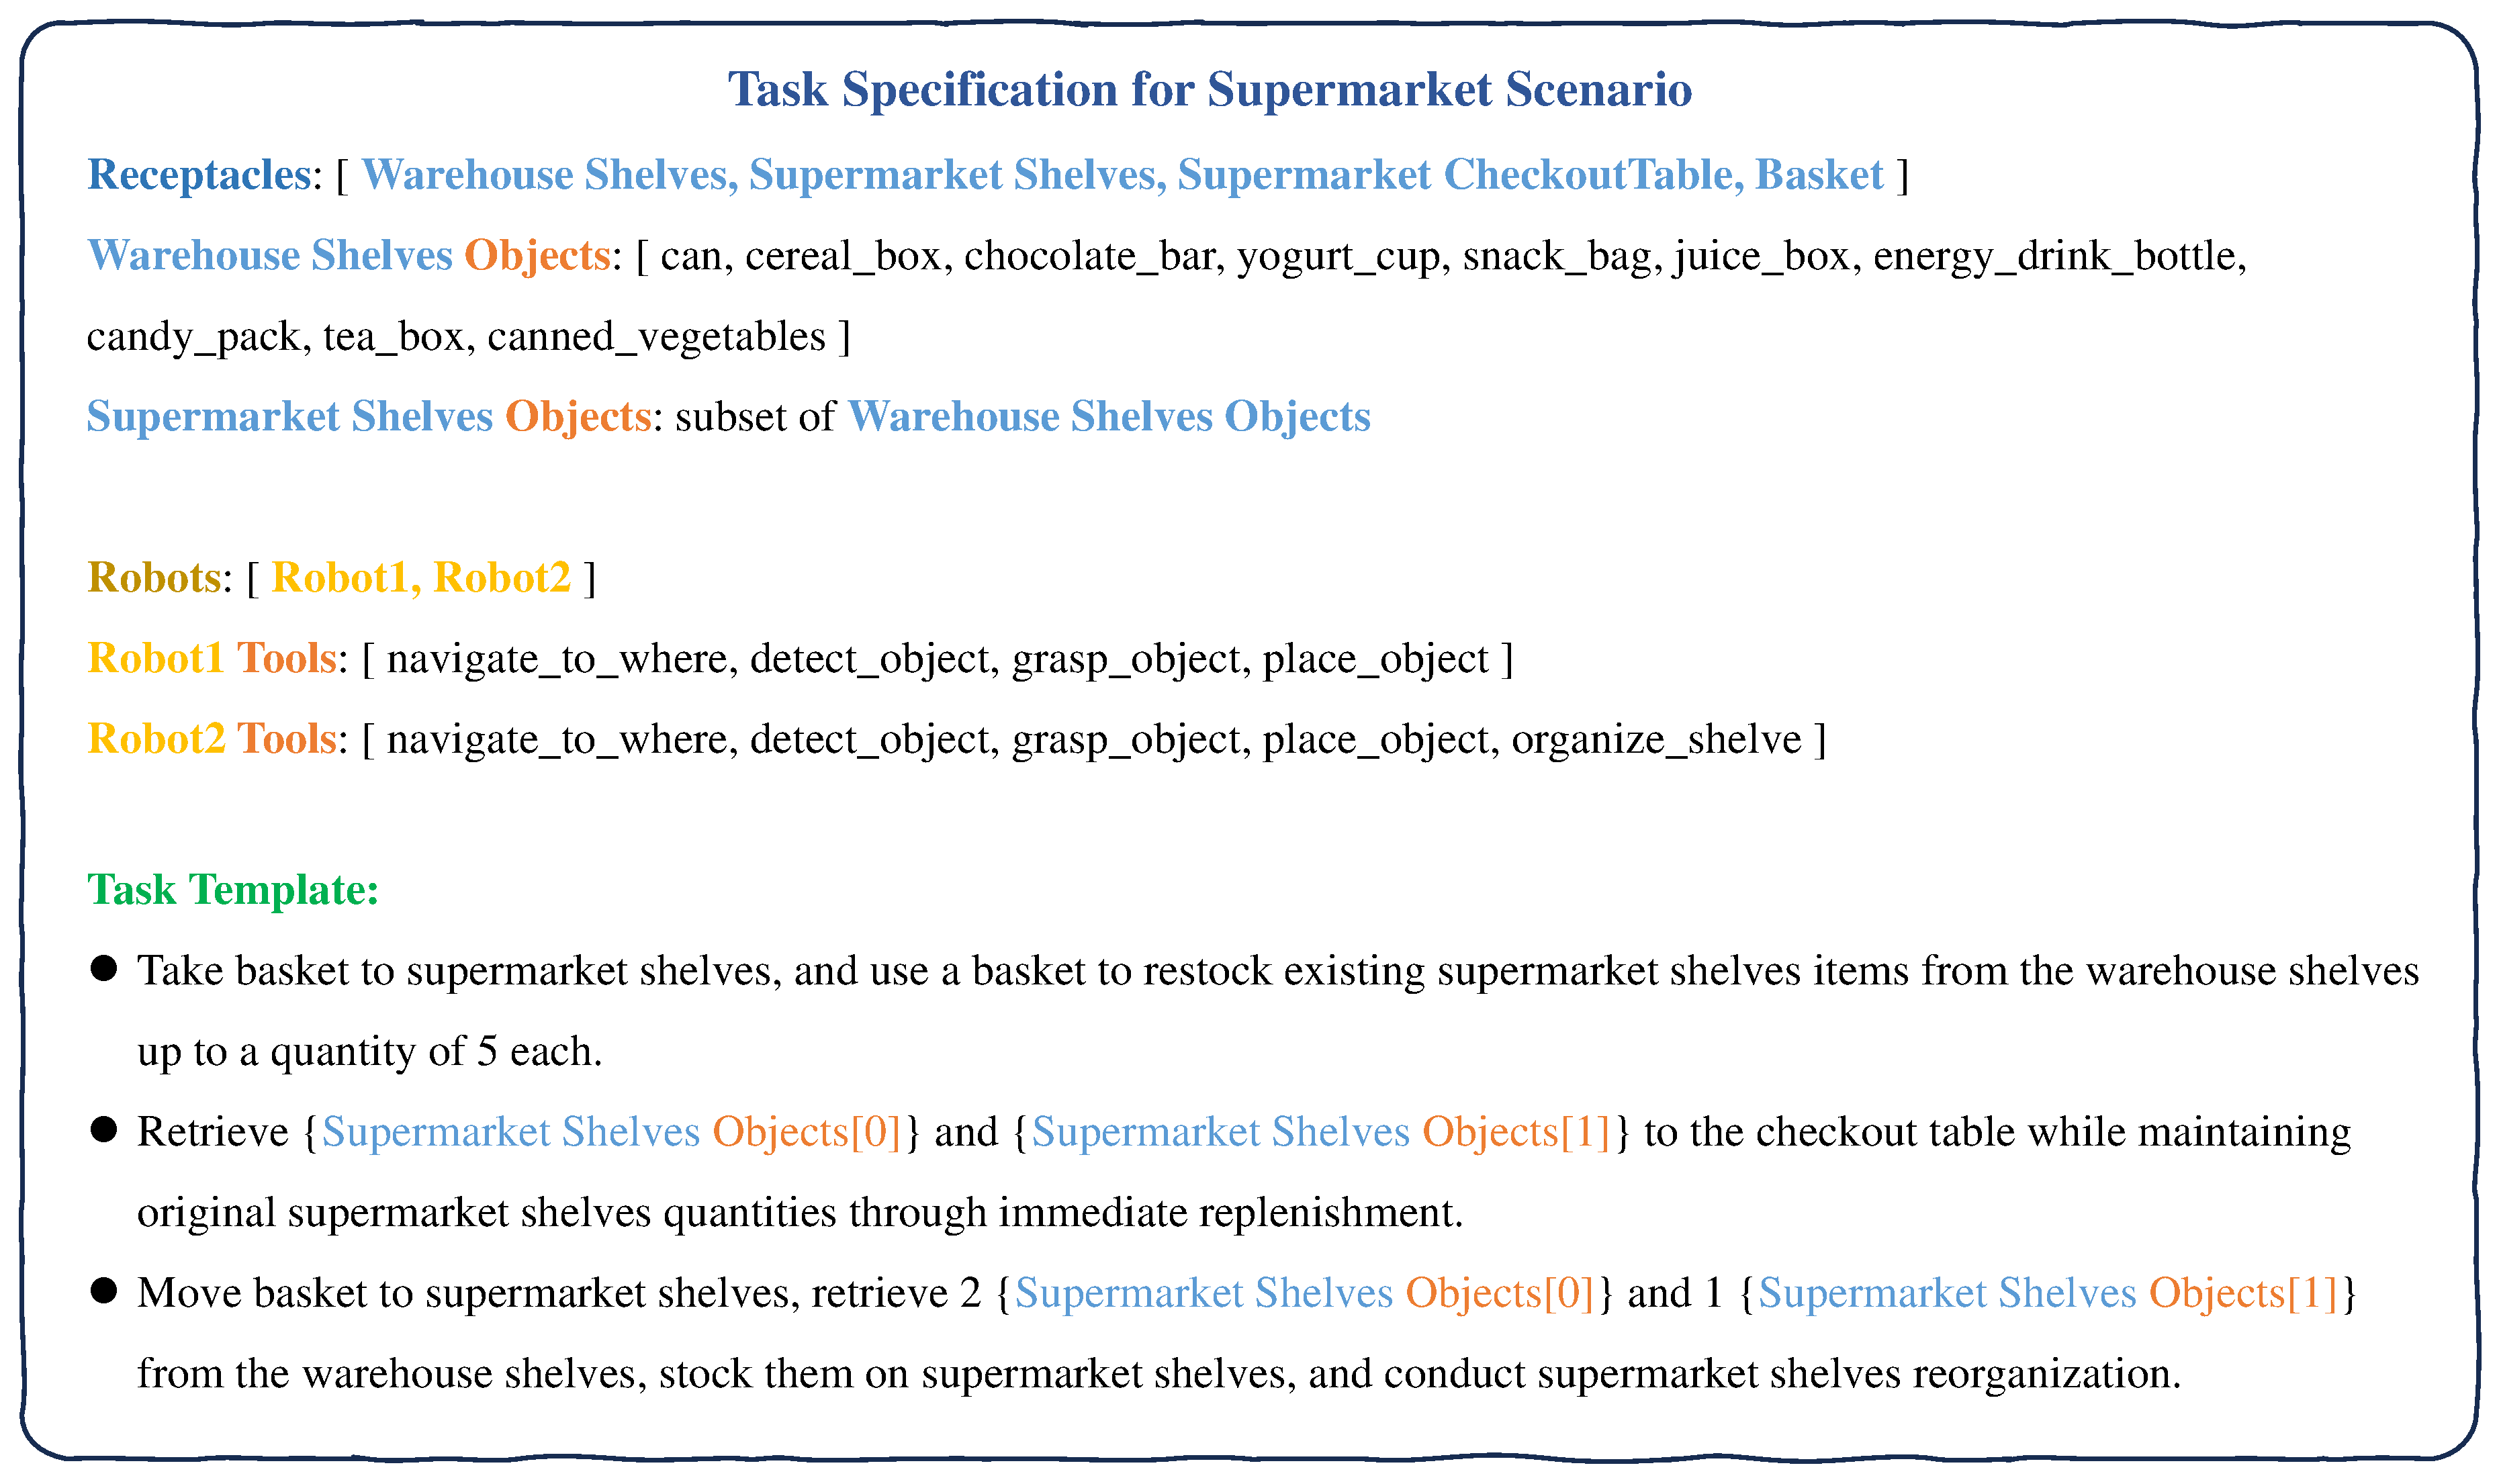
\includegraphics[width=0.94\linewidth]{images/supermarket.pdf}
    \vspace{-0.25cm}
    \caption{
        Task specification for supermarket scenario. 
        }
       \vspace{-0.5cm}
    \label{fig:supermarket}
\end{figure*}


\begin{figure*}[!ht]
    \centering
   \vspace{-0.2cm}
    
\includegraphics[width=0.97\linewidth]{images/prompt_1.pdf}
    \caption{
        Prompt for global task decomposition. 
        }
       \vspace{-0.5cm}
    \label{fig:prompt1}
\end{figure*}

\begin{figure*}[!ht]
    \centering
   \vspace{-0.2cm}
    
\includegraphics[width=0.97\linewidth]{images/prompt_2.pdf}
    \caption{
        Prompt for agent-based tool calling. 
        }
       \vspace{-0.5cm}
    \label{fig:prompt2}
\end{figure*}